\section{THỐNG KÊ}
\setcounter{ex}{0}

%%Câu 2:
\begin{ex} Trong các dữ liệu sau, dữ liệu nào \textbf{KHÔNG} phải số liệu:
	\choice
	{\True Những môn học có điểm kiểm tra trên 7đ của An}
	{Cân nặng của trẻ sơ sinh}
	{Chiều cao trung bình của các loại cây thân gỗ}
	{Số học sinh ăn trưa tại trường của các lớp}
\end{ex}

%%Câu 7:
\begin{ex}   
	Một bảng thống kê khối lượng táo bán được trong bốn tháng đầu năm 2020 của một hệ thống siêu thị được trình bày dưới đây
	\begin{center}
		\begin{tabular}{|l|c|c|c|c|}
			\hline Tháng & $1$ & $2$ & $3$ & $4$ \\
			\hline Khối lượng & $10$ & $40$ & $25$ & $20$ \\
			\hline
		\end{tabular}
	\end{center}
	Vấn đề mà hệ thống siêu thị đang điều tra là:
	\choice
	{\True Khối lượng táo bán được của từng tháng trong bốn tháng đầu năm $2020$}
	{Các tháng $1$, $2$, $3$, $4$}
	{Tháng và khối lượng}
	{Khối lượng của hệ thống siêu thị}
\end{ex}

%%Câu 8:
\begin{ex}
	Thân nhiệt (độ C) của bệnh nhân $A$ trong $10$ tiếng theo dõi được ghi lại như sau
	\begin{center}
		\begin{tabular}{|c|c|c|c|c|}
			\hline
			38 & 39 & 40 & 40 & 41 \\
			\hline
			39 & 38 & 37 & $-2$ & 37 \\
			\hline
		\end{tabular}
	\end{center}
	Điểm không hợp lí trong bảng dữ liệu trên là:
	\choice
	{$40$}
	{$41$}
	{$39$}
	{\True $-2$}
\end{ex}

%%Câu 14:
\begin{ex} Danh sách học sinh nhóm 1 của lớp 6A:
	\begin{center}
		\begin{tabular}{|c|l|}\hline
			\textbf{STT}&\textbf{Họ và tên}\\ \hline
			1&Trần Công Danh\\
			\hline
			2&Nguyễn Thị Thanh Thảo\\ \hline
			3&24/10/2018\\ \hline
			4&Phan Võ Anh Khôi\\ \hline
		\end{tabular}\\
	\end{center}
	Bạn số mấy cung cấp thông tin không hợp lí?
	\choice
	{4}
	{\True 3}
	{2}
	{1}
\end{ex}


%%Câu 21:
\begin{ex}
	Điều tra về loài hoa yêu thích nhất của $ 20 $ bạn học sinh lớp 6A1. Bạn lớp trưởng thu được dữ liệu sau
	\begin{center}
		\begin{tabular}{|c|c|c|c|c|c|c|c|c|c|}
			\hline H & H & M & C & C & H & M & D & D & C \\
			\hline L & H & H & C & C & L & C & C & L & M \\
			\hline
		\end{tabular}
	\end{center}
	Viết tắt:: H: Hoa Hồng; M: Hoa Mai; C: Hoa Cúc; Đ: Hoa Đào; L: Hoa Lan. Có bao nhiêu bạn yêu thích Hoa Hồng ?
	\choice
	{$ 6 $}
	{\True $ 5 $}
	{$ 11 $}
	{$ 3 $}
\end{ex}

%%Câu 22:
\begin{ex} Việc tham gia các câu lạc bộ bóng đá, bóng bàn, cầu lông được lấy ý kiến của các bạn trong lớp với điều kiện chỉ được chọn tham gia một trong ba câu lạc bộ (Đ: bóng đá, B: bóng bàn; C: cầu lông). Kết quả khảo sát như sau:
	\begin{center}
		\begin{tabular}{|c|c|c|c|c|c|c|c|c|c|}\hline
			B&C&Đ&Đ&B&B&C&Đ\\ \hline
			Đ&Đ&B&B&Đ&Đ&C&Đ\\ \hline
			B&C&Đ&Đ&B&C&Đ&Đ\\ \hline
		\end{tabular}\\
	\end{center}
	Chọn bảng thống kê tương ứng với bảng dữ liệu trên
	\choice
	{\True \begin{tabular}{|c|c|c|c|c|c|c|c|c|c|}\hline
			Câu lạc bộ&Bóng đá&Bóng bàn&Cầu lông\\ \hline
			Số học sinh&12&7&5\\ \hline
	\end{tabular} }
	{ \begin{tabular}{|c|c|c|c|c|c|c|c|c|c|}\hline
			Câu lạc bộ&Bóng đá&Bóng bàn&Cầu lông\\ \hline
			Số học sinh&10&7&7\\ \hline
	\end{tabular} }
	{ \begin{tabular}{|c|c|c|c|c|c|c|c|c|c|}\hline
			Câu lạc bộ&Bóng đá&Bóng bàn&Cầu lông&Bóng rổ\\ \hline
			Số học sinh&10&5&5&4\\ \hline
	\end{tabular}}
	{ \begin{tabular}{|c|c|c|c|c|c|c|c|c|c|}\hline
			Câu lạc bộ&Bóng đá&Bóng bàn&Cầu lông\\ \hline
			Số học sinh&11&8&5\\ \hline
	\end{tabular}}
\end{ex}


%%Câu 23:
\begin{ex}
	Bạn Nam điều tra về số học sinh giỏi một số môn học của các bạn trong lớp và lập ra bảng sau
	\begin{center} 
		\def\nam{
			\raisebox{-2pt}{\begin{tikzpicture}[>=stealth,line join=round,line cap=round,font=\footnotesize,scale=0.65]
					\foreach \i in {1,2,3,4}
					\draw (0.2*\i,0)--++(90:0.8) (0,0.2)--(1,0.6);
				\end{tikzpicture}\,\,}}
		\def\hai#1{
			\raisebox{-2pt}{\begin{tikzpicture}[>=stealth,line join=round,line cap=round,font=\footnotesize,scale=0.65]
					\foreach \i in {1,...,#1}
					\draw (0.2*\i,0)--++(90:0.8);
				\end{tikzpicture}\,\,}}	
		\def\vetranh#1{\foreach \dem in{1,...,#1}{\nam}}
		%----
		{\renewcommand\arraystretch{1.5} %giãn dòng
			%\def\tenbieudo{Loại quả yêu thích của các bạn học sinh khối 6}
			\def\noidungtrai{Môn học}
			\def\noidungphai{Kiểm đếm}
			\begin{tabular}{|c|l|} 
				%\hline
				%\multicolumn{2}{|c|}{\bf\color{blue} \tenbieudo}\\
				\hline
				\bf \noidungtrai & \multicolumn{1}{|c|}{\bf \noidungphai}\\
				\hline
				Toán&\vetranh{3}\hai{2}\\ \hline
				Văn&\vetranh{1}\hai{4}\\ \hline
				Tiếng Anh&\vetranh{3}\\ \hline
				Khoa học Tự nhiên&\vetranh{2}\hai{4}\\ \hline
			\end{tabular} 
		}\\[2mm]
		(Mỗi \nam~$=5$ bạn; \hai{1}~$=1$ bạn) 
	\end{center}
	Theo bảng trên, môn học nào có ít số học sinh giỏi nhất?
	\choice
	{Toán}
	{Khoa học Tự nhiên}
	{Tiếng Anh}
	{\True Văn}
\end{ex}

%%Câu 25:
\begin{ex}
	Bảng điều tra về số khách hàng ăn các loại kem yêu thích của một tiệm $A$ trong buổi sáng chủ nhật được ghi dưới đây.
	
	\begin{center}
		\begin{tabular}{|c|c|}
			\hline
			\textbf{Loại kem} & \textbf{Kiểm đếm}\\
			\hline 
			Dâu& \begin{tikzpicture}[>=stealth,scale=0.6, line join = round, line cap = round]
				\coordinate (A) at (3,0); 
				\coordinate (B) at (3.4,0); 
				\coordinate (C) at (3.8,0); 
				\coordinate (D) at (4.2,0);  
				\coordinate (F) at (3,1.4); 
				\coordinate (G) at (3.4,1.4); 
				\coordinate (H) at (3.8,1.4); 
				\coordinate (I) at (4.2,1.4); 
				\coordinate (M) at (2.8,0.4);
				\coordinate (N) at (4.4,1.2);  
				
				\coordinate (A1) at (5.1,0); 
				\coordinate (B1) at (5.5,0); 
				\coordinate (C1) at (5.9,0); 
				\coordinate (D1) at (6.3,0);
				\coordinate (F1) at (5.1,1.4); 
				\coordinate (G1) at (5.5,1.4); 
				\coordinate (H1) at (5.9,1.4); 
				\coordinate (I1) at (6.3,1.4); 
				\coordinate (M1) at (4.9,0.4);
				\coordinate (N1) at (6.6,1.2);  
				
				\coordinate (A2) at (7,0); 
				\coordinate (F2) at (7,1.4); 
				\draw (A)--(F);
				\draw (B)--(G);
				\draw (C)--(H);
				\draw (D)--(I);
				\draw (M)--(N);
				\draw (A1)--(F1);
				\draw (B1)--(G1);
				\draw (C1)--(H1);
				\draw (D1)--(I1);
				\draw (M1)--(N1);
				\draw (A2)--(F2);
			\end{tikzpicture}  \\
			\hline 
			Nho & \begin{tikzpicture}[>=stealth,scale=0.6, line join = round, line cap = round]
				\coordinate (A) at (3,0); 
				\coordinate (B) at (3.4,0); 
				\coordinate (C) at (3.8,0); 
				\coordinate (D) at (4.2,0);  
				\coordinate (F) at (3,1.4); 
				\coordinate (G) at (3.4,1.4); 
				\coordinate (H) at (3.8,1.4); 
				\coordinate (I) at (4.2,1.4);
				\draw (A)--(F);
				\draw (B)--(G);
				\draw (C)--(H);
				\draw (D)--(I);
			\end{tikzpicture} \\
			\hline
			Sầu riêng & \begin{tikzpicture}[>=stealth,scale=0.6, line join = round, line cap = round]
				\coordinate (A) at (3,0); 
				\coordinate (B) at (3.4,0); 
				\coordinate (C) at (3.8,0); 
				\coordinate (D) at (4.2,0);
				\coordinate (F) at (3,1.4); 
				\coordinate (G) at (3.4,1.4); 
				\coordinate (H) at (3.8,1.4); 
				\coordinate (I) at (4.2,1.4); 
				\coordinate (M) at (2.7,0.4);
				\coordinate (N) at (4.5,1.2);  
				
				\coordinate (A1) at (5.1,0); 
				\coordinate (B1) at (5.5,0); 
				\coordinate (C1) at (5.9,0); 
				\coordinate (F1) at (5.1,1.4); 
				\coordinate (G1) at (5.5,1.4); 
				\coordinate (H1) at (5.9,1.4); 
				\draw (A)--(F);
				\draw (B)--(G);
				\draw (C)--(H);
				\draw (D)--(I);
				\draw (M)--(N);
				\draw (A1)--(F1);
				\draw (B1)--(G1);
				\draw (C1)--(H1);
			\end{tikzpicture} \\
			\hline
			Sô cô la & \begin{tikzpicture}[>=stealth,scale=0.6, line join = round, line cap = round]
				\coordinate (A) at (3,0); 
				\coordinate (B) at (3.4,0); 
				\coordinate (C) at (3.8,0); 
				\coordinate (D) at (4.2,0); 
				\coordinate (F) at (3,1.4); 
				\coordinate (G) at (3.4,1.4); 
				\coordinate (H) at (3.8,1.4); 
				\coordinate (I) at (4.2,1.4); 
				\coordinate (M) at (2.7,0.4);
				\coordinate (N) at (4.5,1.2);  
				\draw (A)--(F);
				\draw (B)--(G);
				\draw (C)--(H);
				\draw (D)--(I);
				\draw (M)--(N);
			\end{tikzpicture} \\
			\hline
			Va ni &  \begin{tikzpicture}[>=stealth,scale=0.6, line join = round, line cap = round]
				\coordinate (A) at (3,0); 
				\coordinate (B) at (3.4,0);   
				\coordinate (F) at (3,1.4); 
				\coordinate (G) at (3.4,1.4);  
				\draw (A)--(F);
				\draw (B)--(G);
			\end{tikzpicture} \\
			\hline
		\end{tabular}
	\end{center}
	Có bao nhiêu khách hàng ăn kem dâu ?
	\choice
	{$ 6 $}
	{$ 10 $}
	{\True $ 11 $}
	{$ 8 $}
\end{ex}


%%Câu 26:
\begin{ex} Cho bảng thống kê về thời gian tự học ở nhà của bạn An như sau:
	\begin{center}
		\begin{tabular}{|c|c|c|c|c|c|c|c|}\hline
			\textbf{Ngày trong tuần}&Thứ 2&Thứ 3&Thứ 4&Thứ 5&Thứ 6 &Thứ 7&Chủ nhật \\ \hline
			\textbf{Thời gian (phút)} &80&100&60&80&120&90&0\\ \hline
		\end{tabular}\\
	\end{center}
	Ngày nào trong tuần An dành thời gian tự học ở nhà nhiều nhất?
	\choice
	{Thứ hai}
	{Thứ ba}
	{\True Thứ sáu}
	{Thứ bảy}
\end{ex}

%%Câu 28:
\begin{ex}
	Bảng dữ liệu ghi số xe ô tô bán được của cửa hàng A
	\begin{center}
		\begin{tabular}{|c|c|c|c|c|c|c|} \hline
			\textbf{Năm} & $2015$ & $2016$ & $2017$ & $2018$ & $2019$ & $2020$ \\ \hline
			\textbf{Số xe bán} & $40$ & $30$ & $50$ & $85$ & $75$ & $90$ \\ \hline
		\end{tabular}
	\end{center}	
	Năm nào bán được nhiều xe ô tô nhất?
	\choice{$2017$}
	{$2019$}
	{$2018$}
	{\True $2020$}
\end{ex}

%%Câu 30:
\begin{ex}
	Kết quả kiểm tra thường xuyên môn Toán của học sinh lớp $6A_9$ được cho trong bảng sau:
	\begin{center}
		\begin{tabular}{|c|c|c|c|c|c|c|c|c|c|c|}
			\hline
			Điểm & 1 & 2 & 3 & 4 & 5 & 6 & 7 & 8 & 9 & 10 \\ 	
			\hline
			Số Học sinh & 0 & 1 & 0 & 3 & 8 & 8 & 9 & 4 & 6 & 4 \\ 	
			\hline		
		\end{tabular}
	\end{center}	
	Số học sinh đạt điểm trung bình trở lên (từ điểm $5$ trở lên) là
	\choice
	{$8$}
	{$43$}
	{\True $39$}
	{$4$}
\end{ex}

%%Câu 32:
\begin{ex}
	Điểm Toán của tổ $1$ lớp 6A được cho bởi bảng sau
	\begin{center}
		\begin{tabular}{|c|c|c|c|c|c|c|}
			\hline Điểm&9&8&7&6&5&4\\
			\hline Số học sinh đạt&6&4&7&3&2&6\\
			\hline
		\end{tabular}
	\end{center}
	Bao nhiêu học sinh đạt điểm $6$?
	\choice
	{$1$}
	{$2$}
	{\True $3$}
	{$4$}
\end{ex}

%%Câu 36:
\begin{ex}
	Tình hình sản xuất của một phân xưởng lắp ráp xe ô tô trong một tuần được biểu diễn trong biểu đồ sau. Nhận xét nào sau đây là đúng?
	\begin{center}
		\begin{tabular}{|c|l|}
			\hline 
			Ngày & Số xe lắp ráp được\\
			\hline 
			Thứ Hai & 
			\begin{tabular}{l}
				\tikz{
					\foreach \i in {0,1,2,3,4,5}
					\node (\i) at (\i *1.5,0) {\twemoji[height=1cm]{blue_car}};  
				}
			\end{tabular}
			\\ 
			\hline 
			Thứ Ba & 
			\begin{tabular}{l}
				\tikz{
					\foreach \i in {0,1,2,3,4,5,6}
					\node (\i) at (\i *1.5,0) {\twemoji[height=1cm]{blue_car}};  
				}
			\end{tabular}
			\\
			\hline
			Thứ Tư &
			\begin{tabular}{l}
				\tikz{
					\foreach \i in {0,1,2}
					\node (\i) at (\i *1.5,0) {\twemoji[height=1cm]{blue_car}};  
					\clip (4.25,-0.5) rectangle (4.85,0.25); 
					\node (x) at (4.5,0) {\twemoji[height=1cm]{blue_car}};
				}
			\end{tabular}
			\\
			\hline
			Thứ Năm & 
			\begin{tabular}{l}
				\tikz{
					\foreach \i in {0,1,2,3,4,5,6}
					\node (\i) at (\i *1.5,0) {\twemoji[height=1cm]{blue_car}};  
				}
			\end{tabular}
			\\
			\hline
			Thứ Sáu &
			\begin{tabular}{l}
				\tikz{
					\foreach \i in {0,1,2,3,4,5}
					\node (\i) at (\i *1.5,0) {\twemoji[height=1cm]{blue_car}};  
				}
			\end{tabular}
			\\
			\hline 
			Thứ Bảy & 
			\begin{tabular}{l}
				\tikz{
					\foreach \i in {0,1,2,3,4}
					\node (\i) at (\i *1.5,0) {\twemoji[height=1cm]{blue_car}};  
					\clip (7.25,-0.5) rectangle (7.85,0.25); 
					\node (x) at (7.5,0) {\twemoji[height=1cm]{blue_car}};
				}
			\end{tabular}
			\\
			\hline
		\end{tabular}
		
		\begin{tikzpicture}[>=stealth,line join=round,line cap=round,font=\footnotesize,scale=1]
			\node (a) at (0,0) {\twemoji[height=1cm]{blue_car}};
			\node (b) at (1.6,-0.2) {$10$ xe ô tô};
			\begin{scope}[xshift=4cm]
				\begin{scope}
					\clip (-0.5,-0.5) rectangle (0.1,0.25); 
					\node (c) at (0,0) {\twemoji[height=1cm]{blue_car}};
				\end{scope}
				\node (d) at (1.3,-0.2) {$5$ xe ô tô};
			\end{scope}
		\end{tikzpicture}
	\end{center}
	\choice
	{\True Thứ Năm sản xuất nhiều hơn Thứ Tư $45$ xe ô tô}
	{Thứ Năm sản xuất ít hơn Thứ Tư $55$ xe ô tô}
	{Thứ Năm sản xuất nhiều hơn Thứ Tư $55$ xe ô tô}
	{Thứ Năm sản xuất ít hơn Thứ Tư $45$ xe ô tô}
\end{ex}

%%Câu 39:
\begin{ex}
	Dữ liệu về loại quả yêu thích của các bạn học sinh khối lớp $6$ được cho bởi bảng sau
	\begin{center}
		\begin{tabular}{|c|p{7cm}<{}|}\hline 
			\textbf{Loại quả}&\centerline{\textbf{Số học sinh yêu thích}}\\ \hline 
			Táo&\twemoji[scale=0.8]{star}	\twemoji[scale=0.8]{star}\tikz{\clip(-.5,-.4)rectangle(0,.3);\path(0,0)node{\twemoji[scale=0.8]{star}};}	\\ \hline 
			Chuối&\twemoji[scale=0.8]{star}	\twemoji[scale=0.8]{star}\twemoji[scale=0.8]{star}	\twemoji[scale=0.8]{star}\twemoji[scale=0.8]{star}	\\ \hline 
			Dưa hấu&\twemoji[scale=0.8]{star}	\twemoji[scale=0.8]{star}\twemoji[scale=0.8]{star}\twemoji[scale=0.8]{star}	\twemoji[scale=0.8]{star}\twemoji[scale=0.8]{star}\twemoji[scale=0.8]{star}	\\ \hline 
			Cam&\twemoji[scale=0.8]{star}	\twemoji[scale=0.8]{star}\twemoji[scale=0.8]{star}	\twemoji[scale=0.8]{star}\tikz{\clip(-.5,-.4)rectangle(0,.3);\path(0,0)node{\twemoji[scale=0.8]{star}};}	\\ \hline 
			Bưởi&\twemoji[scale=0.8]{star}	\twemoji[scale=0.8]{star}\twemoji[scale=0.8]{star}	\twemoji[scale=0.8]{star}\twemoji[scale=0.8]{star}\twemoji[scale=0.8]{star}	\\ \hline 
		\end{tabular}\\
		\twemoji[scale=.5]{star} = 10 học sinh;	\tikz{\clip(-.5,-.25)rectangle(0,.5);\path(0,0)node{\twemoji[scale=.5]{star}};} = 5 học sinh
	\end{center}
	Em hãy cho biết tổng số học sinh lớp $6$ thích ăn dưa hấu và cam là bao nhiêu?
	
	\choice
	{$120$}
	{\True $115$}
	{$12$}
	{$11{,}5$}
	
\end{ex}


%%Câu 40:
\begin{ex}
	\begin{figure}[htbp]
		\begin{minipage}[c]{0.6\linewidth}
			\begin{flushleft}
				Biểu đồ tranh sau đây biểu diễn số lượng học sinh Tổ 3 lớp 6B sử dụng các phương tiện khác nhau để đi đến trường. Số học sinh đến trường bằng xe máy (ba mẹ chở) nhiều hơn số học sinh đến trường bằng xe đạp là
			\end{flushleft}
		\end{minipage}
		\begin{minipage}[c]{0.4\linewidth}
			\begin{center}
				\begin{tabular}{|p{9em}|p{6em}|}
					\hline
					Đi bộ & \twemoji[scale=0.6]{1f9d1-1f3fb}\\
					\hline
					Xe đạp&\twemoji[scale=0.6]{1f9d1-1f3fb} \twemoji[scale=0.6]{1f9d1-1f3fb} \\
					\hline
					Xe máy(ba mẹ chở)&\twemoji[scale=0.6]{1f9d1-1f3fb} \twemoji[scale=0.6]{1f9d1-1f3fb} \twemoji[scale=0.6]{1f9d1-1f3fb} \\
					\hline
					Phương tiện khác& \twemoji[scale=0.6]{1f9d1-1f3fb}\\
					\hline
				\end{tabular}\\
				(Mỗi \twemoji[scale=0.6]{1f9d1-1f3fb} ứng với $2$ học sinh)
			\end{center}
		\end{minipage}
	\end{figure}		
	\choice
	{$0$ học sinh}
	{$1$ học sinh}
	{\True $2$ học sinh}
	{$3$ học sinh}
\end{ex}





%%Câu 50:
\begin{multicols}{2}
	\begin{minipage}{9cm}
		\begin{ex} Biểu đồ cột sau cho biết số quyển tập trắng được quyên góp cho học sinh khó khăn. Trong đó, số quyển tập được quyên góp của khối 6 là:
			\choice
			{\True 200 quyển}
			{250 quyển}
			{150 quyển}
			{300 quyển}
		\end{ex}
	\end{minipage}
	\hfill
	\begin{minipage}{9cm}
		\begin{center}
			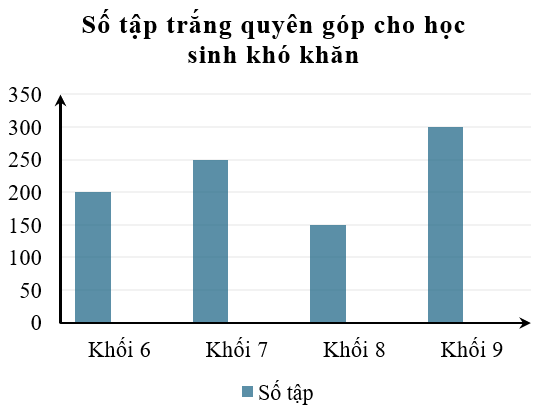
\includegraphics[scale=0.45]{data/Hình/C26_Tk_K6.png}
		\end{center}
	\end{minipage}
\end{multicols}




%%Câu 42:
\begin{ex} Biểu đồ tranh sau đây biểu diễn số lượng máy cày của 5 xã. Em hãy cho biết xã B có bao nhiêu nhiêu máy cày?
	\begin{center}
		\def\icon{\twemoji[scale=0.7]{tractor}}
		\def\hicon{\tikz{\clip(-.4,-.5)rectangle(0,.7);\path(0,0)node{\twemoji[scale=1]{tractor}};}}
		\def\vetranh#1{\foreach \dem in{1,...,#1}{\icon \ }}{
			\begin{tabular}{|c|p{8cm}<{}|}\hline 
				\bf Xã&\multicolumn{1}{c|}{\bf Số máy cày}\\ \hline 
				A&\vetranh{4}\\ \hline 
				B&\vetranh{4}\ \hicon \\ \hline 
				C&\vetranh{2}\ \hicon \\ \hline 
				D&\vetranh{5}\\ \hline 
				E&\vetranh{3}\ \hicon \\ \hline 
			\end{tabular}\\
			\icon = 10 chiếc;        \hicon = 5 chiếc}
	\end{center}
	\choice
	{$40$}
	{50}
	{35}
	{\True 45}
\end{ex}

%%Câu 46:
\begin{ex} 
	Cho biểu đồ tranh về số học sinh khối $6$ được điểm $10$ trong tuần. Chọn kết quả \textbf{SAI}.
	\begin{center}
		\begin{tabular}{|c|c|}
			\hline
			\textbf{Ngày} & \textbf{Số học sinh được $10$ điểm}\\
			\hline
			Thứ Hai & \scalebox{1.3}[1.3]{\faSmile}\quad \scalebox{1.3}[1.3]{\faSmile}\quad \scalebox{1.3}[1.3]{\faSmile}\\
			\hline
			Thứ Ba & \scalebox{1.3}[1.3]{\faSmile}\quad \scalebox{1.3}[1.3]{\faSmile}\\
			\hline
			Thứ Tư &  \scalebox{1.3}[1.3]{\faSmile}\\
			\hline
			Thứ Năm & \scalebox{1.3}[1.3]{\faSmile}\quad \scalebox{1.3}[1.3]{\faSmile}\quad \scalebox{1.3}[1.3]{\faSmile}\quad \scalebox{1.3}[1.3]{\faSmile}\quad \scalebox{1.3}[1.3]{\faSmile}\\
			\hline
			Thứ Sáu & \scalebox{1.3}[1.3]{\faSmile}\quad \scalebox{1.3}[1.3]{\faSmile}\quad \scalebox{1.3}[1.3]{\faSmile}\\
			\hline
		\end{tabular}\\[3mm]
		
		(\scalebox{1.3}[1.3]{\faSmile}\ $=10$ học sinh)
	\end{center}
	\choice
	{Thứ $5$ có số học sinh đạt điểm $10$ nhiều nhất}
	{Thứ $4$ có số học sinh đạt điểm $10$ ít nhất}
	{\True Thứ $3$ và thứ $6$ bằng nhau}
	{Thứ $2$ có $30$ học sinh đạt điểm $10$}
	
\end{ex}


%%Câu 48: 
\begin{ex}
	Biểu đồ dưới đây cho biết số lượng sách giáo khoa lớp 6 bán được tại một hiệu sách vào ngày Chủ nhật vừa qua. Tổng số cuốn sách giáo khoa lớp 6 mà hiệu sách bán được trong ngày Chủ nhật vừa qua là bao nhiêu cuốn?
	
	\begin{center}
		\begin{tabular}{|c|l|}
			\hline
			\multicolumn{2}{|c|}{Số học sinh đạt điểm 10 môn toán lớp 6A}\\
			\hline
			Toán & \faBook~ \faBook ~\faBook~\faBook~\faBook~\faBook~\faBook  \\
			\hline
			Ngữ văn  & \faBook~\faBook~\faBook~\faBook  \\
			\hline
			Tin học & \faBook~ \faBook \\
			\hline
			Lịch sử và Địa lý & \faBook~ \faBook \\
			\hline
			Khoa học tự nhiên &  \faBook~ \faBook ~\faBook~\faBook~\faBook~\faBook\\
			\hline
		\end{tabular}\\
		Mỗi \faBook~ ứng với $9$ cuốn sách.
	\end{center}
	Tổng số cuốn sách giáo khoa lớp 6 mà hiệu sách bán được trong ngày Chủ nhật vừa qua là bao nhiêu cuốn?
	\choice
	{\True $189$}
	{$210$}
	{$190$}
	{$180$}
\end{ex}





%%Câu 51:
\begin{ex}
	Quan sát biểu đồ cột dưới đây rồi chọn khẳng định đúng.
	\begin{center}
		\begin{tikzpicture}[scale=0.6, font=\footnotesize, line join=round, line cap=round,>=stealth, local bounding box=BieuDo]
			%Gán số liệu.
			\def\xmax{10};\def\ymax{5};\def\donvi{2};
			\definecolor{mau}{HTML}{2faabb};
			%Gán tọa độ.
			\coordinate (O) at (0,0);
			%Trục Oxy.
			\draw[->, thick] (O)--(\xmax,0);
			\draw[->, thick] (O)--(0,\ymax);
			\foreach \giatri [count=\index] in {0,2,4,6,8,10}{
				\draw[mau, thick, opacity=0.5] (0,\index-1)--(\xmax,\index-1);
				\fill (0,\index-1) node[left]{$\giatri$} circle(1pt);
			}
			\foreach \x/\y/\giatri/\noidung [count=\index] in {2/2.5/5/{Lan},4/3/6/{Hoa},6/4.5/9/{Đào},8/4.5/9/{Hồng}}{
				\fill[mau] (\x-0.3,0) rectangle (\x+0.3,\y);
				\draw (\x,0)node[below]{\noidung};
			}
			%Tiêu đề biểu đồ.
			\draw ($(BieuDo.north)+(90:0.5)$) node{\bfseries Điểm đầu năm học};
		\end{tikzpicture}
	\end{center}
	\choice
	{\True Điểm đầu năm học của Hoa là $6$ điểm}
	{Điểm đầu năm học của Lan cao hơn điểm đầu năm học của Hoa}
	{Điểm đầu năm học của Hồng là $10$ điểm}
	{Điểm đầu năm học của Đào thấp hơn điểm đầu năm học của Hồng}
	
\end{ex}


%%Câu 53:
\begin{ex} 
	\immini
	{
		Quan sát biểu đồ bên, thôn nào thu hoạch được nhiều thóc nhất?
		\choice
		{Thôn Đông}
		{Thôn Trung}
		{\True Thôn Nam}
		{Thôn Bắc}
	}
	{
		\begin{tikzpicture}[>=stealth,line join=round,line cap=round,font=\footnotesize,scale=0.6]
			\def\tl{5}
			\def\kc{.5}
			\foreach \n in {1,2,...,6}{
				\pgfmathsetmacro{\ny}{int(\n*\tl)}
				\draw[opacity=.3,dashed] (0,\n)
				node[left,opacity=1]{$\ny$}
				--++(0:8);
			}
			\foreach \x/\y [count=\i from 0] in {12/Bắc,18/Trung,24/Nam,21/Đông}
			{
				\pgfmathsetmacro{\ni}{\i*2+1}
				\pgfmathsetmacro{\xi}{\x/\tl}
				\fill[orange!50,draw] ({\ni-\kc/2},0) rectangle +(\kc,\xi);
				\draw (\ni,2pt)--(\ni,-2pt)
				node[below]{\y}
				;
				\path (\ni,\xi)node[above]{\x};
			}
			\draw[<->] (0,6.5)|-(8,0)
			;
			\fill circle (1pt) node[left]{$O$};
			\draw (current bounding box.north) node[align=center]{\textbf{Số thóc của bốn thôn thu hoạch năm 2015}\\\textit{(tấn)}};
		\end{tikzpicture}
	}
\end{ex}

%%Câu 54:
\begin{ex} Biểu đồ cột sau thể hiện loại học lực của các học sinh khối 6 của trường THCS Star.
	\begin{center}
		\begin{tikzpicture}
			[scale=0.6,font=\small,line join=round,>=stealth]
			\def\hoanh{10.2};
			\def\tung{4.2};
			\node[above] at (\hoanh/2,\tung+1){\normalsize \bfseries Xếp loại học lực học sinh khối 6};
			\def\mau{mauChuDao};
			\draw (0,0)node[left]{0}--(\hoanh,0);
			\draw[->] (0,0)--(0,\tung+1);
			\foreach \y in {20,40,...,160}{\draw (-0.1,\y/35)node[left]{$\y$}--++(0:0.2);
				\draw[dashed,gray] (0,\y/35)--(\hoanh-0.2,\y/35);}
			\foreach \x/\n in{2/38,4/140,6/52,8/13}{\draw[line width=7mm,\mau] (\x,0)--++(0,\n/35)node[black,shift={(90:0.3)}]{\n};}
			\foreach \x/\p in {2/Giỏi,4/Khá,6/Trung bình,8/Yếu}{\node at (\x,-0.4){\footnotesize \p};} 
		\end{tikzpicture}
	\end{center}
	Số lượng học sinh học lực trung bình ít hơn số lượng học sinh học lực khá là:
	\choice
	{192}
	{\True 88}
	{102}
	{98}
\end{ex}

%%Câu 56:
\begin{ex} Cho biểu đồ sau:
	\begin{center}
		\begin{tikzpicture}[scale=0.6,font=\small,line join=round,>=stealth]
			\def\hoanh{11.2};
			\def\tung{4.5};
			\node[above] at (\hoanh/2,\tung+1.2){\normalsize \bfseries Ước tính dân số Việt Nam qua các thập niên};
			\node[above] at (\hoanh/2,\tung+0.6){\normalsize (triệu người)};
			\def\mau{mauChuDao};
			\draw[->] (0,0)node[left]{0}--(\hoanh,0);
			\draw[->] (0,0)--(0,\tung+1);
			\foreach \y in {20,40,...,120}{\draw (-0.1,\y/25)node[left]{$\y$}--++(0:0.2);
				\draw[dashed,gray] (0,\y/25)--(\hoanh-0.2,\y/25);}
			\foreach \x/\n in{1/53,3/67,5/79,7/87,9/93}{\draw[line width=4mm,\mau] (\x,0)--++(0,\n/25)node[above,black]{\n};}
			\foreach \x/\p in {1/1979,3/1989,5/1999,7/2009,9/2019}{\node at (\x,-0.4){\footnotesize \p};} 
		\end{tikzpicture}
	\end{center}
	Dân số Việt Nam từ năm 1989 đến năm 2009 tăng:
	\choice
	{87 triệu dân}
	{8 triệu dân}
	{40 triệu dân}
	{\True 20 triệu dân}
\end{ex}

%%Câu 57:
\begin{ex} Điểm thi của Nam và Khải được biểu diễn trong biểu đồ cột kép ở hình sau:
	\begin{center}
		\begin{tikzpicture}[scale=1,font=\small,line join=round,>=stealth]
			\def\hoanh{7.2};
			\def\tung{4.7};
			\def\mau{mauChuDao};
			\draw[->] (0,0)node[left]{0}--(\hoanh,0)node[below]{Môn học};
			\draw[->] (0,0)--(0,\tung+1);
			\foreach \y in {1,2,...,10}{\draw (-0.1,\y/2)node[left]{$\y$}--++(0:0.2);
				\draw[dashed,gray] (0,\y/2)--(\hoanh-0.2,\y/2);}
			\foreach \x/\n/\p in{1/7/10,3/8/6,5/9/8}{
				\draw[line width=5mm,\mau] (\x-0.25,0)--++(0,\n/2);
				\draw[line width=5mm,cyan] (\x+0.25,0)--++(0,\p/2);}
			\foreach \x/\p in {1/Toán,3/Ngữ Văn,5/Tiếng Anh}{\node at (\x,-0.4){\footnotesize \p};}        
			\fill[\mau] (1.5,\tung+1) rectangle (2,\tung+1.3) node [black,shift={(-10:0.6)}]{Nam};
			\fill[cyan] (3.5,\tung+1) rectangle (4,\tung+1.3) node [black,shift={(-10:0.6)}]{Khải};
		\end{tikzpicture}
	\end{center}
	Khẳng định nào sau đây \textbf{đúng}:
	\choice
	{Điểm Toán của Nam cao hơn Khải}
	{Điểm cả 3 môn của Khải cao hơn Nam}
	{\True Điểm Ngữ văn của Nam cao hơn Khải}
	{Điểm Tiếng Anh của Khải cao hơn Nam}
\end{ex}


%%Câu 59:
\begin{ex} Cho biểu đồ cột kép sau:
	\begin{center}
		\begin{tikzpicture}[scale=0.8,font=\small,line join=round,>=stealth]
			\def\hoanh{10.2};
			\def\tung{4.7};
			\node[above] at (\hoanh/2,\tung+1){\normalsize \bfseries Số con vật được học sinh tổ 3 và tổ 4 nuôi};
			\def\mau{mauChuDao};
			\draw (0,0)node[left]{0}--(\hoanh,0);
			\draw[->] (0,0)--(0,\tung+1);
			\foreach \y in {2,4,...,16}{\draw (-0.1,\y/3)node[left]{$\y$}--++(0:0.2);
				\draw[dashed,gray] (0,\y/3)--(\hoanh-0.2,\y/3);}
			\foreach \x/\n/\p in{1/8/4,3/5/5,5/10/2,7/12/15,9/5/2}{
				\draw[line width=5mm,\mau] (\x-0.3,0)--++(0,\n/3);
				\draw[line width=5mm,cyan] (\x+0.3,0)--++(0,\p/3);}
			\foreach \x/\p in {1/Chó,3/Mèo,5/Chim,7/Cá,9/Thỏ}{\node at (\x,-0.4){\footnotesize \p};}        
			\fill[\mau] (2.5,-1) rectangle (3,-1.3) node [black,shift={(10:0.7)}]{Tổ 3};
			\fill[cyan] (5,-1) rectangle (5.5,-1.3) node [black,shift={(10:0.7)}]{Tổ 4};
		\end{tikzpicture}
	\end{center}
	Số con cá của tổ 3 và tổ 4 nuôi trong biểu đồ ở hình trên là:
	\choice
	{Tổ 3 là 10, tổ 4 là 14}
	{Tổ 3 là 12, tổ 4 là 14}
	{\True Tổ 3 là 12, tổ 4 là 15}
	{Tổ 3 là 15, tổ 4 là 12}
\end{ex}	

